% Template Credit to:
% A. Thall, 2003
% R. Roos, 2013
% G. Kapfhammer, 2017
% OBC, 2018

\NeedsTeXFormat{LaTeX2e}
\documentclass[12pt]{report}


% use varepsilon
\DeclareSymbolFont{epsilon}{OML}{ntxmi}{m}{it}
\DeclareMathSymbol{\epsilon}{\mathord}{epsilon}{"0F}

%\usepackage[bottom,single]{gatorthesis} % for final department copy
\usepackage[debug,draft,single]{gatorthesis} % for student workcopy
%\usepackage[single]{gatorthesis} % for student
%\usepackage[debug,draft,nolists,nofront,single]{gatorthesis} % more options

\usepackage{comment}
\usepackage{amsmath}
\usepackage{amssymb}
\usepackage{epsfig}
\usepackage{url}
\usepackage{listings}
\usepackage[figure]{algorithm2e}
\usepackage{graphicx}

% custom packages
\usepackage{fancyhdr}
\usepackage{hyperref}
\usepackage{subcaption}
\usepackage{mathtools}
\usepackage[utf8]{inputenc}
\usepackage[T1]{fontenc}
\usepackage{mathptmx}



% Don't hyphenate the words "itself" or "linear". Hyphenate
%          "representations" only at the places indicated by the "-":
\hyphenation{itself repre-sen-tations linear}

% custom commands
\newcommand{\name}{{\sc RayTerm}}
\newcommand{\rayorg}{\vec{R_{origin}}}
\newcommand{\raydir}{\vec{R_{direction}}}

\newcommand\todo[1]{
\begin{center}
  \color{red}
  {\bf TODO}\\
  #1
\end{center}
}

\begin{document}

\thesistitle{{\large \name:}\\{A Ray-Tracing Rendering Engine\\for XTerm-like Terminals}}

\thesisauthor{Saejin Mahlau-Heinert} \thesisadvisor{Dr. Janyl Jumadinova}

\thesisnumber{CS-2019-10}

\thesisreadera{Dr. Gregory Kapfhammer}

\date{\FileRevised \\ $\mbox{}$Revision: 1.8 $\mbox{}$}

\thesismaketitle
\thesismakecopyright

%   ********************************************************************
%   * YOU MAY SPLIT YOUR THESIS INTO SEVERAL FILES AND "\include" THEM *
%   * AS SHOWN BELOW. FOR INSTANCE, FILE "abstract.tex" CONTAINS THE   *
%   * ABSTRACT, FILE "ack.tex" CONTAINS THE ACKNOWLEDGMENTS, ETC. YOU  *
%   * MAY, OF COURSE, PUT EVERYTHING INTO ONE HUGE FILE, BUT THERE ARE *
%   * ADVANTAGES TO SPLITTING THINGS UP--FOR EXAMPLE, YOU CAN COMMENT  *
%   * OUT "\include" LINES OF SOME PARTS IN ORDER TO PRINT DRAFTS      *
%   * CONTAINING SELECTED SECTIONS OF YOUR THESIS, SAVING PAPER AND    *
%   * PRINTING COSTS.                                                  *
%   *                                                                  *
%   * YOU ARE NOT REQUIRED TO HAVE A "dedication"--IF YOU DON'T, JUST  *
%   * DELETE THAT LINE OR COMMENT IT OUT WITH A LEADING "%"            *
%   ********************************************************************

\begin{abstract}
  Over the many years of innovation in the field of computer graphics, advances in rendering have led to massive increases in the fidelity of engaging, satisfying, and realistic computer visualizations.
  \name{} is a new and unique entry into the ranks of rendering engines, and makes its own contributions to the field of computer graphics.
  While harkening back to the retro aesthetics of the seventies and eighties, \name{} embraces new advances in computing power to bring path-traced photorealistic visuals to an old screen\,---\,the terminal.
  Using Unicode block characters to simulate pixels and a single-branch path-tracer written in C++ and CUDA, \name{} renders a fully three-dimensional scene, complete with global illumination and physically-based materials.
  \name{} can be used as an engine for terminal-based tools, visualizations, games, and more; it is fully open-source and ready for integration or use within other projects.

\end{abstract}
  % REQUIRED!

% \include{dedication} % OPTIONAL

% \include{ack}       % OPTIONAL, BUT ALMOST EVERYONE INCLUDES IT

%   ********************************************************************
%   * FRONT MATTER--TABLE OF CONTENTS, ETC. YOU PROBABLY DON'T NEED TO *
%   * CHANGE ANY OF THIS UNLESS YOU HAVE NO TABLES OR FIGURES, OR YOU  *
%   * WANT TO CHANGE NUMBERING DEPTH FOR SUBSECTIONS, OR ...           *
%   ********************************************************************

\setcounter{tocdepth}{2}    % # of section levels shown in table of contents
\setcounter{secnumdepth}{3} % # of numbered subsection levels in the text

\tableofcontents
%\listoftables       % OMIT THIS IF YOU DON'T HAVE ANY TABLES
\listoffigures      % OMIT THIS IF YOU DON'T HAVE ANY FIGURES

%   ********************************************************************
%   * A GLOSSARY IS ALMOST NEVER NEEDED UNLESS YOU HAVE AN UNUSUALLY   *
%   * LARGE NUMBER OF SPECIAL TERMS OR NOTATIONS AND IT WOULD DETRACT  *
%   * TOO MUCH FROM THE FLOW OF THE PAPER TO DEFINE THEM IN-LINE.      *
%   ********************************************************************
%\include{glossary}  % OMIT THIS IF YOU DON'T HAVE A GLOSSARY (FEW PEOPLE DO)

%   ********************************************************************
%   * THE FOLLOWING "lstset" COMMAND IS ADAPTED FROM ONE FOUND AT:     *
%   * http://tex.stackexchange.com/questions/115467/                   *
%   * listings-highlight-java-annotations                              *
%   *                                                                  *
%   * SEE CHAPTER 3 AND APPENDIX A                                     *
%   ********************************************************************

\lstset{
  basicstyle=\footnotesize\tt, % the size of the fonts that are used for the code
  breakatwhitespace=false,     % automatic breaks only happen at whitespace?
  breaklines=true,             % sets automatic line breaking
  captionpos=b,                % sets the caption-position to bottom
  frame=single,                % adds a frame around the code
  language=Java,               % the language of the code
  keywordstyle=\bf,
  showspaces=false,
  showstringspaces=false,      % underline spaces within strings only?
  showtabs=false,
  tabsize=2                    % sets default tabsize to 2 spaces
}

%   ********************************************************************
%   * NOW INCLUDE THE CHAPTER FILES; COMMENT OUT ANY YOU DON'T WANT TO *
%   * PROCESS IN A PARTICULAR LATEX RUN.                               *
%   *                                                                  *
%   * INCLUDED FILES ARE ASSUMED TO END IN ".tex", E.G.,               *
%   * "ch01_overview.tex", "ch02_relatedwork.tex", ETC.                *
%   ********************************************************************

% ch:intro
%
% $Id: ch01_overview
%
%   *******************************************************************
%   * SEE THE MAIN FILE "AllegThesis.tex" FOR MORE INFORMATION.       *
%   *******************************************************************

\chapter{Introduction}
\label{ch:intro}

In the early days of computing, real-time rendering engines that powered games like ``Doom'' or ``NetHack'' had to run on extremely underpowered hardware and render on low-resolution screens.
The dream of real-time, photorealistic graphics was far, far away.
However, even then the simple, blocky graphics, easily recognizable shapes, and maze-like environments were fantastic entertainment.
Today the retro-style of low-resolution graphics, pixel art, and 8-bit color abounds in the gaming space.
\name\ is one part of enabling that retro-aesthetic to grow into a new and unique style that, while similar to the old classics, can be more engaging and real than they ever were.

This thesis document describes a system that creates a moving image on a terminal screen.
This system is called \name; it performs real-time updating of the displayed image, thus generating a window into a three-dimensional (3D) world.
\name\ is available for a wide variety of other programs to use as a rendering engine.
With the current generation of powerful computers, able to execute billions or even trillions of calculations per second, it is finally possible to do real-time, close-to-photorealistic rendering.
While the goal of \name\ is not high-resolution photorealism, some approximation is achieved.

In this introduction to \name, we will first cover the motivations behind creating this system in Section~\ref{ch:intro:motivation}.
Then, we will give an overview of the project in Section~\ref{ch:intro:overview}.
Section~\ref{ch:intro:background} expands on the overview to provide some mathematical grounding for some of the algorithms used in \name.
In Section~\ref{ch:intro:background:development_ecosystem} we cover the main development tools used in this project, such as the implementation language.
Finally, Section~\ref{ch:intro:outline} outlines the rest of this thesis document, introducing the major topics of discussion for the remaining chapters.

\section{Motivation}
\label{ch:intro:motivation}

I have always been fascinated with rendering algorithms, especially ray-tracing.
This fascination fueled an interest in game engine development, 3D modeling, and other computer graphics topics.
The idea for \name\ came out of a disappointment -- I was working on a project that made a virtual space seem larger than it was when the user was wearing a virtual reality headset.
Sadly, someone had already developed a toolkit that did exactly what I wanted to achieve.

Through my search for a replacement project, I discovered that, for me, one of the biggest draws to an idea was the ability for that idea to affect other people.
Whether it was something that many others could use or an idea that people could contribute to, I wanted to make something other people saw.
That is where the draw of open-source software came from for me, and why \name\ is open-source.
Additionally, I discovered that there are many niches in software -- places where there just is not a lot of people making things.
Computer graphics in a terminal emulator (see Section~\ref{ch:intro:overview:ncurses}) is one of those corners.
The only real application many people saw for this niche was the rendering of images to the terminal -- in fact, some of the initial inspiration for \name\ came from TerminalImageViewer \cite{tivGithub}, a program to accomplish that very task.

I saw more possibilities, however.
There is no need to keep the terminal in a by-gone era, stuck with only colored characters and still graphics.
The terminal is, after all, only a window into some text.
Why does this text have to be stationary?
Why does it need to be text at all?
The answer, of course, is that it does not.
There is a huge amount of potential in a 3D rendering engine that outputs to the terminal -- there are so many applications, from rendering 3D model files to playing video games to visualizing music.
All that these programs need is an infrastructure around the terminal for 3D rendering.
\name\ aims to create that infrastructure through a completely novel combination of ray-traced 3D rendering and Unicode-based image composition.

\section{Overview}
\label{ch:intro:overview}

\name\ uses the recursive ray-tracing algorithm, simulating the path of light through the scene -- this is described in more detail in Section~\ref{ch:intro:overview:raytracing}.
Many images are generated, or rendered, each second; once an image is rendered the \texttt{ncurses} library \cite{ncursesLibrary} is used to display it in a terminal.
Multiple images are displayed in quick succession, creating the illusion of movement.
More details on this process are given in Section~\ref{ch:intro:overview:ncurses}.
Rendered images are displayed in two different modes; the first uses single half-character pixels, and the second more complex Unicode block characters.
The mechanics of these image composition methods are discussed in Section~\ref{ch:intro:overview:unicode}.
Finally, Figure~\ref{fig:checker_metal} is a still image of the final terminal output \inlinetodo{update with actual output image}.

\begin{figure}[htb]
  \centering
  \includegraphics[width=0.8\textwidth]{resources/checker_metal}
  \caption{Example of terminal output}
  \label{fig:checker_metal}
\end{figure}

\subsection{Rendering Engines and Ray-Tracing}
\label{ch:intro:overview:raytracing}

A rendering engine is an algorithm that takes a scene -- a description of some collection of objects -- and generates an image or visual representation of that scene.
There are many different algorithms that accomplish this goal.
\name\ utilizes the recursive ray-tracing algorithm first pioneered by Turner Whitted in his ground-breaking paper ``An Improved Illumination Model for Shaded Display'' \cite{whitted1980improved}.
Ray-tracing was one of the first algorithms developed in the field of computer graphics, and although there have been some improvements since then, the idea behind the algorithm has maintained its original simplicity.

Ray-tracing has been used as the rendering algorithm of choice for photorealistic scenes because with only a few modifications to Whitted's original algorithm, it can generate fantastic images.
In the past, however, render times have been so slow that it was impossible to generate images fast enough for real-time use.
For example, Figure~\ref{fig:povray_render} is a render created by the POV-Ray engine \cite{povray}.
POV-Ray can take between a few minutes to several hours to complete one single image depending on the processing power involved.
However, there have been a few recent innovations that change this, such as NVIDIA's RTX hardware acceleration.
Section~\ref{ch:intro:background:hardware} provides more details on these advances and how \name\ takes advantage of them.

\begin{figure}[htb]
  \centering
  \includegraphics[width=0.8\textwidth]{resources/glasses_povray}
  \caption{POV-Ray render created by Gilles Tran \cite{povray2006render}}
  \label{fig:povray_render}
\end{figure}

Ray-tracing revolves around the idea of {\it rays}, a mathematical construct that represents an infinite line emanating in some direction from a starting point in three-dimensional space.
In \name\, rays are used to simulate the path that light takes as it travels around the scene.
When a ray intersects with an object in the scene various interactions take place that simulate how light may travel under different conditions.
It is worth noting that a base assumption is made in ray-tracing when using straight rays as described here: light follows a straight line without changes.
This is only the case in reality when light travels through a vacuum with no gravitational bodies; thus, basic ray-tracing is not exactly photorealistic and does not model phenomena like atmospheric scattering.
Additional mathematics and systems must be used to bend, attenuate, or scatter a ray to accurately render transparent volumes -- this is called volumetric ray-tracing.
Volumetric ray-tracing is not currently supported in \name, but is a fascinating area for future work.

The formal basis for ray-tracing is the rendering equation, articulated by James Kajiya in 1986 \cite{kajiya1986rendering}.
The rendering equation models the outgoing light at some point in some direction given all incoming light, a bidirectional reflectance distribution function (BDRF), and a normal (a perpendicular direction) for the surface at the point modeled.
If solved for every point in the scene, the rendering equation could generate a completely photorealistic image -- this would, however, require massive amounts of computation.
This is because the rendering equation contains an integral over all incoming light which must be solved through numerical analysis.
Ray-tracing algorithms that do this are known as {\it path-tracers} and are the most photorealistic rendering algorithms invented.

\name\ does not use a path-tracer -- such algorithms are still many times too slow for most real-time rendering situations.
Instead, the rendering equation is solved by sampling the incoming light at each point with rays.
This is known as recursive ray-tracing since it starts with a single ray that splits every time it encounters a surface.
The eventual goal of the recursive ray-tracing algorithm is to create a tree of rays for each {\it fragment} to render.
A fragment is either a pixel or some sub-pixel -- many systems will use four or more fragments per pixel to get better anti-aliasing and more accurate results.
Each ray contains some color that represents the color of the light in that ray.
When a ray hits an object, it is {\it scattered} by the {\it material} of the object, splitting and generating new rays.
These rays are biased towards directions that contain lots of incoming light -- such as towards a point light source.
The specific implementation of recursive ray-tracing that \name\ uses only scatters into a set number of rays at each intersection point: one ray toward each light source, along with reflection and refraction rays towards the relevant directions \inlinetodo{update with relevant scatter numbers}.

The base of each generated tree is an {\it eye-ray} -- a ray with its origin at the fragment location on the camera plane.
The eye-ray's color is the color that will be rendered for that fragment.
As the eye-ray projects forward, away from the eye, it is tested for intersection with all objects in the scene.
When an intersection happens and the generated rays scattered, the eventual color values of the scattered rays are combined to produce the color of the original eye-ray.
This is done recursively to fully render the scene.

\subsection{Terminal Output using \texttt{ncurses}}
\label{ch:intro:overview:ncurses}

Output in \name\ is shown in a terminal window.
A terminal is a specific kind of interface for a computer that uses text-based commands and feedback, as opposed to a Graphical User Interface (GUI).
It descends from the old days of mainframe computers, where the actual computer was not under a desk -- instead, users would connect over a network to the main computer, using an actual terminal machine.
Today, the terminals most people use are actually ``terminal emulators'', because they simply emulate these old mainframe terminal machines.
These terminal emulators are often simply programs that run in an existing graphical desktop environment, providing a text-based interface to the operating system.

Once an image is generated, \name\ must somehow display that image in a terminal with no surrounding prompt or other formatting -- as a simple {\it character field}.
To do this, we use a two-step approach: first, we represent the image using Unicode characters (see Section~\ref{ch:intro:overview:unicode}), then we print those characters to the terminal using a C library called \texttt{ncurses} \cite{ncursesLibrary}.
This library abstracts implementation details of the terminal to enable full-window 24-bit color character output.
% TODO: update with actual fps
In \name, the terminal window is divided into two ``panels'', a main panel for the actual image output -- updated 30 times or more per second -- and an info panel to render information such as frames per second and logging text.
Additionally, extra terminal output such as the command prompt or other character output is disabled.

The main problems that \texttt{ncurses} solves are ones which need to use terminal escape codes -- short character sequences that tell a terminal emulator to change some specific data or use a different display method.
These escape codes will tell the terminal how to display text by changing the formatting, positioning, or color.
The library can also disable character ``echoing'', the display of characters that are typed by the user.
Because of this dependency on \texttt{ncurses}, \name\ can be used only with terminals that support it -- generally, any XTerm-like terminal will work, as long as it supports a terminal information database: either \texttt{termcap} or \texttt{terminfo} \cite{ncursesLibrary}.

\subsection{Image Composition using Unicode Characters}
\label{ch:intro:overview:unicode}

Unicode is a character standard that allows anyone to reference many thousands of characters to compose text, no matter the environment around the text \cite{unicode}.
Some critical characters that \name\ uses are known as the {\it block characters} -- they are characters \texttt{U+2580} -- \texttt{U+259F}, a subset of which are shown in Figure~\ref{fig:unicode_characters}.
The core of image composition using Unicode is an algorithm coloring the characters and the background -- \name\ uses this algorithm on every character of the output to both determine the character to display, and the foreground and background colors for that character.
The foreground colors the character itself, whereas the background provides a relief color.
This allows each {\it character~pixel} to represent a hard gradient.

\begin{figure}[htb]
  \centering
  \hspace{0.3em}
  \begin{subfigure}[htb]{0.4\textwidth}
    \includegraphics[width=\textwidth]{resources/block_elements}
    \caption{Block Elements}
    \label{fig:unicode_block_characters}
  \end{subfigure}
  \hfill
  \begin{subfigure}[htb]{0.51\textwidth}
    \includegraphics[width=\textwidth]{resources/quadrant_elements}
    \caption{Quadrant Elements}
    \label{fig:unicode_quadrant_characters}
  \end{subfigure}
  \caption{Subset of \texttt{U+2580} -- \texttt{U+259F} \cite{unicode}}
  \label{fig:unicode_characters}
\end{figure}

There are two image modes available for use in \name.
The first is pure {\it pixel mode}, in which the Unicode ``half-block'' symbol (\texttt{U+2584}) is used.
Since monospaced character output (such as in a terminal) is twice as tall as it is wide, the half-block can split a single character into two pixels that are colored differently: the upper pixel with the background color of the character, and the lower with the character or foreground color of the pixel.
This means that a typical 85 by 30 character terminal results in a screen space of 85 by 60 pixels.
This mode also dramatically reduces the number of ray-tracing computations needed, since only one ray per pixel is required.

The second image mode is considerably more complicated and slower, as it uses significantly more rays per character in order to determine what Unicode block character most fits the desired output.
On the other hand, it allows a much higher perceived resolution, since the characters used have smaller footprints of down to an eighth of a character in width or length.
The differences between these two modes are highlighted in Figure~\ref{fig:unicode_mode_comparison1} and~\ref{fig:unicode_mode_comparison2} \inlinetodo{update with actual output}.
It can be seen that the first image mode, {\it pixel mode}, shows a rather fuzzy definition of the main large sphere.
However, in the second image mode, {\it character mode}, the sphere and the reflections seen in it are much more defined.
The performance impact of both modes is another factor that was assessed when making implementation decisions for \name; it informed how much actual definition was added by the second rendering mode.
With the current implementation, there is around a four-fold decrease in performance \inlinetodo{update with actual decrease in performance}.

\begin{figure}[htb]
  \centering
  \begin{subfigure}[htb]{0.49\textwidth}
    \includegraphics[width=\textwidth]{resources/many_spheres_square}
    \caption{Pixel Mode Image Output}
    \label{fig:unicode_mode_comparison1}
  \end{subfigure}
  \hfill
  \begin{subfigure}[htb]{0.49\textwidth}
    \includegraphics[width=\textwidth]{resources/many_spheres}
    \caption{Character Mode Image Output}
    \label{fig:unicode_mode_comparison2}
  \end{subfigure}
  \caption{Examples of Image Mode Output}
  \label{fig:unicode_mode_comparison}
\end{figure}

\section{Background}
\label{ch:intro:background}

The background information for the algorithms and techniques used to implement \name\ is discussed in this section.
We introduce basic vector mathematics in Section~\ref{ch:intro:background:vector_math}.
In Section~\ref{ch:intro:background:raytracing_math} we detail most of the specific mathematical algorithms involved.
In \name, many of these algorithms are implemented behind the scene in APIs like OptiX and CUDA \inlinetodo{update with actual implementation location}.

\subsection{Vector Mathematics}
\label{ch:intro:background:vector_math}

Vector mathematics is a way to represent operations on $n$-dimensional constructions.
The main unit of computation is a vector -- essentially, a list of $n$ numbers.
A vector is denoted with an arrow over its name: $\vec{v} = (-2, 3, 1)$ is a vector.
A specific value in a vector is referenced by either its zero-based index, $\vec{v}_{0}$ is the first value in $\vec{v}$ (note the arrow is above $v$ only, and not the index), or its dimension -- $\vec{v}_x$ is the same value.
The dimensions are by convention $x$, $y$, $z$, and $w$.
In \name\ however, we generally work only with vectors where $n = 3$ (only in $x$, $y$, and $z$), and each vector represents either a direction or a position in three-dimensional space.
Vectors are related to both multivariable calculus and linear algebra -- an expansion on this basic explanation can be found in virtually any textbook on these topics.

\littlesection{Vector Operations}

Each set of all possible $n$-dimensional vectors are closed under the basic arithmetic operations.
Addition, subtraction, along with some specialized versions of multiplication, are all defined.
Addition and subtraction are calculated on a component-wise basis -- for instance, in three dimensions addition and subtraction can be calculated using Formulas \ref{equation:vector_addition} and \ref{equation:vector_subtraction}.

\begin{equation}
  \label{equation:vector_addition}
  \vec{u} + \vec{v} = (\vec{u}_x + \vec{v}_x, \vec{u}_y + \vec{v}_y, \vec{u}_z + \vec{v}_z)
\end{equation}

\begin{equation}
  \label{equation:vector_subtraction}
  \vec{u} - \vec{v} = (\vec{u}_x - \vec{v}_x, \vec{u}_y - \vec{v}_y, \vec{u}_z - \vec{v}_z)
\end{equation}

There are three other operations, each based on numerical multiplication.
The first is simple scalar multiplication.
A scalar in this context is just a regular number, such as $2$.
Scalar multiplication is defined by Formula~\ref{equation:vector_scalar_multiplication}, and is also a closed operation for $n$-dimensional vectors.

\begin{equation}
  \label{equation:vector_scalar_multiplication}
  k\vec{v} = (k\vec{v}_x, k\vec{v}_y, k\vec{v}_z)
\end{equation}

Then we have the cross product.
This is a specialized multiplication operation only applicable when $n = 3$ that results in a vector that is perpendicular to both of its operands.
The cross product of $\vec{u}$ and $\vec{v}$ is denoted as $\vec{u} \times \vec{v}$, and can be calculated with Formula~\ref{equation:vector_cross_product}.

\begin{equation}
  \label{equation:vector_cross_product}
  \vec{u} \times \vec{v} = (\vec{u}_y\vec{v}_z - \vec{u}_z\vec{v}_y, \vec{u}_z\vec{v}_x - \vec{u}_x\vec{v}_z, \vec{u}_x\vec{v}_y - \vec{u}_y\vec{v}_x)
\end{equation}

Finally, the dot product is a third multiplication operation that is applicable to any $n$-dimensional vector.
However, the result of the dot product operation is a simple scalar, not a new vector.
The dot product only makes semantic sense when talking about direction vectors: it gives a sense of how much two vectors are ``aligned'' with each other.
It is often used to determine if two vectors are at right angles with each other, since in that case the dot product would be $0$.
The dot product of $\vec{u}$ and $\vec{v}$ is denoted as $\vec{u} \bullet \vec{v}$, and can be found using Formula~\ref{equation:vector_dot_product}.

\begin{equation}
  \label{equation:vector_dot_product}
  \vec{u} \bullet \vec{v} = \vec{u}_x\vec{v}_x + \vec{u}_y\vec{v}_y + \vec{u}_z\vec{v}_z
\end{equation}

\littlesection{Vector Equations}

With the operations described above, we can write equations using vectors.
This greatly simplifies the description of the mathematics in Section~\ref{ch:intro:background:raytracing_math}, since without vector mathematics every operation would need to be notated in cartesian coordinates.
It should be noted that exponentiation for vectors is calculated on a component-wise basis -- for example, $\vec{(1, 4, 2)}$ squared is $\vec{(1, 16, 4)}$.
This is by convention in graphics programming since it provides an easy description of such an operation.
This is not, however, always the case in other mathematical applications of vectors.

When thinking about the meaning and algorithms behind equations, it is extremely helpful to keep two main facts in mind.
First, {\it crossing} two vectors results in a vector that is at a right angle to each; that is, it gives a normal to the plane in which both original vectors lie.
We should note here that according to only this definition, there are actually two possible answers for each set of operands.
However, only one of these answers is correct; to determine the right one, the ``right-hand rule'' is used.
To use the right-hand rule, point your right hand's index finger in the direction of the first vector, and your middle finger in the direction of the second.
Your thumb will point in the direction of the resulting cross product.
Note that this causes the order of operands to matter -- a different order will produce the opposite direction.

\begin{equation}
  \label{equation:vector_dot_product_cos}
  \vec{u} \bullet \vec{v} = |\vec{u}| \cdot |\vec{v}| \cdot cos(\theta)
\end{equation}

Second, {\it dotting} two vectors multiplies their lengths while keeping in mind their direction -- two vectors perfectly parrallel to each other would have a dot product that was simply their lengths multiplied.
However, two vectors perfectly perpendicular to each other have a dot product of zero.
There is actually a second definition of the dot product (Formula~\ref{equation:vector_dot_product_cos}) that can be a little easier to understand with this context.
In this formula, $\theta$ is the angle between the two operands, and $|\vec{w}|$ is the length of $\vec{w}$.

\subsection{Ray-Tracing Mathematics}
\label{ch:intro:background:raytracing_math}

The mathematical basis for ray-tracing is heavily dependent on understanding vector mathematics -- Section~\ref{ch:intro:background:vector_math} is a short introduction.
The basic mathematical construct used in ray-tracing is called a {\it ray}.
Rays are defined by two vectors: an origin point, referred to as $\rayorg$ for some ray $R$, and a direction, referenced as $\raydir$.
These two vectors together represent a line of infinite length that starts at the origin and projects along the direction.
An important addition to the concept of rays is a point along a ray -- this can be defined by using a third variable, $t$, to represent how far along the ray the point is located.
Therefore, Formula~\ref{equation:point_on_ray} can be used to get the coordinates of such a point in three-dimensional space.
Assuming $\raydir$ is a unit vector, this is the {\it parametric~form} of a ray.

\begin{equation}
  \label{equation:point_on_ray}
  \vec{point} = \rayorg + t\raydir
\end{equation}

With this concept, algorithms can be described to model the interaction between rays and other surfaces.
The algorithms discussed are run millions of times per second in a highly parallelized environment.
Parallelization is a technique for running two or more algorithms simultaneously; therefore even minor optimizations are extremely important since they reduce the overall time to render.
All of the ray-tracing mathematics described here are synthesized from Peter Shirley's excellent ``Ray Tracing in One Weekend'' \cite{shirley2016ray} and the Morgan Kaufmann textbook ``Physically Based Rendering: From Theory to Implementation'' \cite{pharr2016physically}.
Some smaller sections also benefit from ideas in Jean-Colas Prunier's ``Scratchapixel'' \cite{prunier2017triangle}.

Scenes that can be ray-traced must be a collection of surfaces that are mathematically intersectable with a ray.
Any surface that can be defined by an implicit surface definition function, in the form of Function~\ref{equation:surface_equation}, is intersectable with a ray \cite{pharr2016physically}.
In Function~\ref{equation:surface_equation} and for the rest of this section, $\vec{p}$ is a vector representing a point in three-dimensional space.
The implicit surface definition function must have the property that if and only if $f(\vec{p})$ is $0$, then $\vec{p}$ is on the defined surface.
The point of intersection between a ray and a surface defined in this way can be found by solving Equation~\ref{equation:ray_surface_intersection} for $t$ and then using Formula~\ref{equation:point_on_ray} to calculate the coordinates of that point on the ray.
We essentially ask, ``What points along this ray are on the defined surface?'' by passing in all possible points on the ray, parameterized by $t$.

\begin{equation}
  \label{equation:surface_equation}
  f(\vec{p}) = 0
\end{equation}

\begin{equation}
  \label{equation:ray_surface_intersection}
  f(\rayorg + t\raydir) = 0
\end{equation}

In \name, the only surfaces that are supported are spheres, triangles, and infinite planes, since their surface definition functions are mathematically simple \inlinetodo{update for actual supported surfaces}.
A sphere is the simplest three-dimensional object to calculate ray intersection with, and therefore was the first implemented for \name.
In fact, during feasibility testing, much of the math described in this section was implemented by hand in the Go programming language, instead of through existing APIs.

\littlesection{Ray-Sphere Intersection}

The surface definition function of a sphere is Function~\ref{equation:sphere_surface}, with $S$ representing the sphere.
The intersection point between a ray and a sphere is given by solving Equation~\ref{equation:ray_sphere_intersection} for $t$ and then using Formula~\ref{equation:point_on_ray}.
Both of these equations are directly adapted from ``Ray Tracing in One Weekend'' \cite{shirley2016ray}.
Notice that Equation~\ref{equation:ray_sphere_intersection} is quadratic, and the number (and values) of the roots give us the $t$ we want to use.
The smallest positive root corresponds to the point on the ray which first intersects the sphere.
If there are no real roots, then the ray does not intersect the sphere.

\begin{equation}
  \label{equation:sphere_surface}
  f(\vec{p}) = (\vec{p} - \vec{S_{center}})^2 - {S_{radius}}^2
\end{equation}

\begin{equation}
  \label{equation:ray_sphere_intersection}
  (\raydir^2)t^2 + 2(\raydir \bullet (\rayorg - \vec{S_{center}}))t + (\rayorg - \vec{S_{center}})^2 - {S_{radius}}^2 = 0
\end{equation}

\littlesection{Ray-Plane Intersection}

For any two-dimensional object, the plane it lies in is the first shape tested for intersection.
Luckily, ray-plane intersection testing is fairly cheap and straightforward.
The surface definition function of a plane is Function~\ref{equation:plane_surface}, with $P$ representing the plane.
The plane's {\it offset} is a point on the plane, and the plane's {\it normal} is a vector perpendicular to the plane.
The intersection point between a ray and a plane is given by solving Equation~\ref{equation:ray_plane_intersection} for $t$ and then using Formula~\ref{equation:point_on_ray}.
These equations were derived from basic vector math, along with guidance from ``Physically Based Rendering'' \cite{pharr2016physically}.

\begin{equation}
  \label{equation:plane_surface}
  f(\vec{p}) = (\vec{p} - \vec{P_{offset}}) \bullet \vec{P_{normal}}
\end{equation}

\begin{equation}
  \label{equation:ray_plane_intersection}
  (\vec{P_{normal}} \bullet \raydir)t + \vec{P_{normal}} \bullet (\rayorg - \vec{P_{offset}}) = 0
\end{equation}

\littlesection{Ray-Triangle Intersection}

The method for testing intersection with triangles is a bit more complicated than the other tests we've covered so far.
The mathematics for this section are again derived from vector mathematics.
However, Jean-Colas Prunier's ``Scratchapixel,'' an excellent and accessible online resource for 3D rendering \cite{prunier2017triangle}, was also an indispensable guide in facilitating understanding along the way.
First, intersection is tested with the plane the triangle lies in -- this results in a ray-plane intersection point $\vec{Q}$, or no intersection.
Then, if there was an intersection, another test must be performed to detect if $\vec{Q}$ is inside the triangle.
We do this using the ``inside-outside'' method (as suggested by ``Scratchapixel''): test if $\vec{Q}$ is on the left side of each edge.

To conduct the test, we label each triangle vertex $\vec{V_i}$, with $i$ increasing in the counter-clockwise direction.
We then have three triangle vertices: $\vec{V_0}$, $\vec{V_1}$, and $\vec{V_2}$.
We can now use Function~\ref{equation:left_edge_test}: if $f(i) > 0$ for each $i$, then $\vec{Q}$ is inside the triangle.
Otherwise, $\vec{Q}$ is outside the triangle.
Note that in Function~\ref{equation:left_edge_test}, if $i = 3$, then $i = 0$ ($i$ ``wraps'' to only valid values).

\begin{equation}
  \label{equation:left_edge_test}
  f(i) = P_{normal} \bullet ((\vec{V_{i+1}} - \vec{V_i}) \times (\vec{Q} - \vec{V_i}))
\end{equation}

Function~\ref{equation:left_edge_test} can be complicated to visualize, so imagine this: we first form two vectors, both with $\rayorg = \vec{V_i}$.
The first points along the triangle's edge, while the other points towards $\vec{Q}$.
Both of these vectors will be in the plane of the triangle.
Thus, if we cross them, the vector produced will either be away from the plane in the same direction as $\vec{P_{normal}}$, or away from the plane in the opposite direction.
According to the right-hand rule, if the crossed vector is in the same direction as $\vec{P_{normal}}$, then the vector pointing to $\vec{Q}$ is ``to the left'' of the vector pointing towards $\vec{V_{i+1}}$.
We can then calculate the dot product between $\vec{P_{normal}}$ and the crossed vector -- if it is positive then the crossed vector is in the same direction as the normal, and therefore $\vec{Q}$ is to the left of the edge.
One last addendum to this intersection test is the fact that it can be difficult to perform the counter-clockwise numbering of vertices.
We therefore simply expect vertices to be specified in counter-clockwise order.
This is similar to what many other 3D rendering algorithms assume.


\section{Development Ecosystem}
\label{ch:intro:background:development_ecosystem}

\name's development relies on many other systems.
The actual implementation code is hosted on Github, a public platform for projects using the Git version control system.
A continuous integration system called Travis CI \cite{travisci} is used for testing and environment management.
Documentation is handled by \texttt{doxygen} \cite{van2008doxygen} -- all external facing functions, methods, and classes have a minimum of a few sentences of documentation.
More details about the implementation tools are given in Section~\ref{ch:intro:background:languages_and_libraries}; testing hardware and low-level APIs are discussed in Section~\ref{ch:intro:background:hardware}.

\subsection{Programming Languages and Tools}
\label{ch:intro:background:languages_and_libraries}

With a large project such as \name, there are certain choices that must be made from a software development perspective.
These choices inform how the project is modified, built, and eventually executed.
In the case of \name, we used the C++ language \cite{cpp14standard} for main development, and Gradle \cite{gradle} as a build system.

\littlesection{Implementation Language}

The C++ language was used for three main reasons.
First, the language has a huge ecosystem of low-level tools, with interfaces to libraries such as OptiX, CUDA, FORTRAN-implemented mathematics like Blitz++, and much more.
This ensures that no matter the need, there was most likely a library out there that could fill that need.
Secondly, C++ allows low-level C-like programming while keeping abstractions such as objects available.
Lastly, C++ is a reasonably fast language: with no virtual machine, unlike Java or Kotlin, garbage collection is not a burden.
Decades of work have gone into compiler toolchains such as \texttt{g++} and \texttt{clang}, enabling automatic optimizations that would not be possible for newer languages.

\name\ attempts to keep most of its implementation to a C-compatible level, using classes and greater abstractions only as necessary.
This ensures that overhead is minimal, as well as guaranteeing readability for the open source release.
Advanced features of C++ such as templating are avoided so as to keep the knowledge entry barrier low.
Finally, all code in \name's implementation conforms to the Google C++ style guide \cite{googleStyleGuide}.

\littlesection{Build System}

Complex projects can be a nightmare to manage, especially when there are multiple contributors.
Build systems are an important tool that simplify this headache.
An opinionated build system such as Gradle also specifies sensible defaults for most situations, requiring minimal starting configuration.
This is why Gradle was chosen as the build system for \name.
Gradle was used to compile C++ code into an executable for distribution or testing using its Software Model feature.
This feature allows the specification of executables and interdependent components, with sensible default source code and binary locations.
Gradle efficiently manages long linking or dependency lists, without resorting to macro-infested and variable-filled makefiles; it also handles header inclusions seamlessly, without dealing with relative path issues.
Gradle can even automatically retrieve dependencies if they are published as a Maven artifact.
All of these features make ongoing development and maintenance an easier proposition.

\subsection{Hardware}
\label{ch:intro:background:hardware}

There are many implementation issues related to the performance aspects of \name since high performance is a strict requirement for obtaining render times low enough for real-time display.
For the purposes of testing, we use a machine with an Intel Core i7 4770k CPU and NVIDIA Geforce GTX 980Ti GPU.
Only recently has ray-tracing even been able to achieve real-time levels of performance; much of this progress is thanks to advances in GPU technology.
The largest innovator in this space, GPU chip design company NVIDIA, released its RTX series of GPUs that have hardware support for ray-tracing.
RTX hardware spread is slow, however, due to its high early adoption cost.
Therefore we do not focus on RTX hardware; instead, we look to slightly older technologies to provide the implementation backbone; this works well with the existing test hardware, which is a few generations old.

% \todo{future subsection on what hardware API we actually used}
% \todo{future subsection on how we dealt with GPU vs CPU\\and how we built two different implementations}

\section{Thesis Outline}
\label{ch:intro:outline}

In the remaining chapters of this thesis document, we will describe the features of \name, detail more advanced background information, and discuss implementation.
Chapter~\ref{ch:relatedwork} reviews a number of past approaches
to ray-tracing, and provides background for some more advanced ray-tracing algorithms and data structures.
It also describes some tools that we used for \name's initial proposal and testing.
Chapter~\ref{ch:methods} outlines the high-level conceptual algorithms, test tooling, and methods used in this project.
It is complemented by Chapter~\ref{ch:implementation}, which is an in-depth description of \name's implementation, including class and function diagrams and organizational information.
Finally, Chapter~\ref{ch:conclusion} completes this document, describing the future work left to complete, a hope for open-source contributions, and a look back at what the author learned through the experience of developing this project.
 % Introduction -- of course, you can name it anything!

% ch:relatedwork
%
% $Id: ch02_relatedwork
%
%   *******************************************************************
%   * SEE THE MAIN FILE "AllegThesis.tex" FOR MORE INFORMATION.       *
%   *******************************************************************
\chapter{Related Work}
\label{ch:relatedwork}

In this chapter, we will discuss a few related research papers, detail how they informed \name's development, and show the improvements of \name\ over other systems.
First, we will conduct a high-level discussion of the first ray-tracing paper through to basic details on modern-day optimizations.
Following that, we will discuss two Github projects, one of which was a major inspiration for Unicode image composition and the algorithms involved (see Section~\ref{ch:intro:overview:unicode}).

\section{Discovery of Ray-Tracing}
\label{ch:relatedwork:discovery}

\subsection{The First Ray-Tracer}
\label{ch:relatedwork:discovery:first}

The very first ray-tracing algorithm was developed by Arthur Appel in his 1968 paper ``Some techniques for shading machine renderings of solids'' \cite{appel1968some}.
His algorithm is now known as a ray casting algorithm -- it does not follow the approach we described in Section~\ref{ch:intro:overview:raytracing}.
Instead, rays are traced from a point light source to the object being shaded, and a plus symbol of varying size is rendered at that location, depending on the intensity of light at that point.
When a photographic negative is taken, light spots that were not hit by the rays (thereby darkening them) are now ``in shadow'', as the color levels were inverted.
Today, Appel's work is not normally considered a real ray-tracing algorithm.
However, his work informed much of the following research, especially his ideas and mathematics on light intensity.
After Appel's work, there were some commercial applications of ray-tracing in the field of radiosity; ray-tracing was used to track radiation inside tanks at Mathematical Applications Group, Inc (MAGI) \cite{whitted2018explains}.

\subsection{The Breakthrough}
\label{ch:relatedwork:discovery:breakthrough}

The next big entry to the ray-tracing field was Turner Whitted's 1980 paper ``An Improved Illumination Model for Shaded Display'' \cite{whitted1980improved}.
In this groundbreaking and approachable work, Whitted introduced the recursive ray-tracing algorithm we covered in Section~\ref{ch:intro:overview:raytracing}.
Whitted was not the first to use ray-tracing -- Arthur Appel had first pioneered the field over a decade ago, and there were also emerging commercial applications.
Whitted's real contribution was the idea for how to improve ray-tracing so that it could solve the problem of {\it global illumination}.
Global illumination was not yet formalized, but the idea was to somehow gather the effect of all light in the scene on every single point.
This can easily be categorized as taking into account both direct lighting, light coming directly from a source, and indirect lighting, light coming from reflections, refractions, or other non-direct travel methods.

Recursive ray-tracing approximates direct lighting easily, as each encountered point sends a ray to each light in the scene.
Indirect lighting is slightly more difficult -- pure reflection and refraction are easy, but as soon as reflections become more diffuse, and there are many, many directions a point gets lit from, recursive ray-tracing breaks down and path-tracing must take over.
Despite this, ray-tracing was able to achieve remarkably good images, and thus Whitted-style ray-tracing was born.
Even today, any simple recursive ray-tracing algorithms are known as Whitted-style ray-tracers. Indeed, \name\ uses a Whitted-style ray-tracer, with only some small enhancements, such as {\it heuristic emissive sampling}.
Essentially, this sampling adds a new generation method for rays so that when a ray encounters a diffuse reflective surface, we attempt to sample the possible locations for other emissive (light-producing or light-reflecting) objects.
This adds some rudimentary support for area lights and diffuse reflections, although it is still not photorealistic.

One element that is not mentioned in ``An Improved Illumination Model for Shaded Display'', but is in Whitted's retrospective on the paper \cite{whitted2018explains}, is adaptive super-sampling.
This method generates more eye-rays, and therefore more definition, only in fragments that do not have sufficient detail.
This is a relatively simple algorithm: the corners of each pixel provide four sample points creating a ``sample square''.
Then, if each of the four points are sampled relatively close in value, and there isn't a small object visible through the pixel, the average sample is taken from each of the four points.
If the points are not close in value, or there is a small object, then the sample square is subdivided and the process starts again, reusing some old values and calculating new ones.
This method is inherently sequential and adds additional complexity to the ray-tracing algorithm.
Therefore, it is not implemented in the current version of \name; however, it could be a future optimization.
This optimization could, in fact, treat the entire starting canvas as a single sample square, and then refine sample points from there.
Depending on the complexity of the small object test, this could be an improvement.

\subsection{Formalization}
\label{ch:relatedwork:discovery:formalization}

The path to fully photorealistic rendering was blazed soon after Whitted's paper.
The mathematical basis for all of ray-tracing and photorealistic rendering was published by James Kajiya in 1986 \cite{kajiya1986rendering}.
In his paper ``The Rendering Equation'', he articulated a generalization for many different rendering algorithms; this generalization is shown as Equation~\ref{equation:the_rendering_equation} below.
Although the idea behind the rendering equation was not completely new, Kajiya presented it in a form using vector mathematics, especially suited for computer graphics.
The equation also gives direction for more advanced and photorealistic rendering techniques, leading up to path-tracing.

\begin{equation}
  \label{equation:the_rendering_equation}
  I(x, x') = g(x, x') \Big[\epsilon(x, x') + \int_{S} \rho(x, x',x'')I(x', x'')dx''\Big]
\end{equation}

This equation is fairly complex, but a basic and simplified explanation will be given here.
First, we will describe the terms: $I(x, x')$ is related to the intensity of light passing from point $x'$ to point $x$; $g(x, x')$ is a ``geometry'' term; $\epsilon(x, x')$ is related to the intensity of emitted light from $x'$ to $x$; $\rho(x, x',x'')$ is related to the intensity of light scatter from $x''$ to $x$ by a patch of surface at $x'$.
Note that inside the integral is a recursive reference -- this is where we build an entire scene's lighting influence on a single point.
We start with some definitions: $x'$ is the point we just hit with our sample ray, $x$ is the origin of our ray, and $x''$ is a point that we get through further ray-tracing -- it is a point found by reflecting or scattering the impacting ray.
The integral is actually the simplest element in the equation; it samples all possible incoming directions for light (referencing itself recursively), calculates the possible reflection from that light along the outgoing direction back towards $x$, and sums all these reflections up.
The $\epsilon$ term is the amount of light emitted from $x'$.
Finally, the $g$ term is included in Kajiya's original paper, but most other formulations remove it in favor of attenuation terms inside the integral.
Essentially, it controls how the geometry around $x'$ affects the outgoing light.

Since for practical purposes we can't infinitely recurse, we will eventually hit a recursion level when evaluating the rendering equation.
In this case, the incoming light is simply set to the ambient light level and no additional recursive calculations take place.
This takes care of all reflection, refraction, and light travel; notice, however, that we must solve the integral over an entire sphere of directions, and we must do this for every single point we sample, for every single direction we sample from.
This is {\it horrendously} inefficient. The significant part of this equation for \name\ is the integral, since if we can approximate that, \name\ would be photorealistic.

In \name, we use the rendering equation to inform the recursive ray generation, attempting to find areas of the integral where most of the light is incoming; this method we name {\it heuristic emissive sampling} (also mentioned above in Section~\ref{ch:relatedwork:discovery:breakthrough}).
In the common case, all light will be from the direction of nearby light sources.
However, we can also bias newly generated rays towards areas where refracted light may exist, such as around glass materials.
Keeping this mathematical basis in mind was critical during implementation since the further we stray from this equation, the less photorealistic the final rendered images become.

\section{Optimizations}

\subsection{Accelerated Intersections}

Ray-tracing requires intersection tests with every object in the scene.
If it were possible to drastically reduce the number of tests computed for each ray, perhaps by only testing the ray against objects in its general vicinity, massive speed increases would emerge.
As it turns out, this was first explored right after Whitted's original paper.
The Bounding Volume Hierarchy (BVH) acceleration structure was proposed in Steven Rubin and Turner Whitted's 1980 paper ``A 3-dimensional representation for fast rendering of complex scenes'' \cite{rubin1980}.

A BVH essentially groups objects into hierarchical organizations, with each group covering a larger area than the groups inside it.
Each group has a {\it bounding volume}, a geometric primitive that encloses all members of that group.
Ray-tracing intersections are done with the root group's bounding volume first, then progress down the hierarchy and potentially skip the vast majority of geometry in the scene, thereby speeding up computation.
There have been numerous improvements to this idea; however, BVHs continue to be an easy-to-implement and efficient acceleration structure \cite{prunier2017bvh}.
A simple BVH was implemented in \name\ \inlinetodo{update with actual structure used}.

\subsection{Parallelization}

Ray-tracing is inherently parallelizable because each eye-ray and its descendants are independent -- rays cannot collide, and one fragment's eye-ray does not affect another fragment's eye-ray.
Thus, there have been many optimizations that target enhanced hardware acceleration to enable massively parallel ray-tracing.
The first example of this was ``Design and Analysis of a Parallel Ray Tracing Computer'' \cite{cleary1983design}, a 1983 paper by John Cleary and others.
In it, Cleary describes a computing system that is functionally similar to the Graphics Processing Units (GPUs) available today.
They were even able to build small prototypes, but calculated that a full-blown system would cost \$50 million and be able to generate 1000 by 1000 pixel images in 0.15 seconds.
Sadly, 1983 chip technology had not yet progressed to the point where such a large multi-core processor was feasible.

However, all is not lost.
Much of the research done in this area led to the design of systems such as OptiX and CUDA, enabling projects like \name\ to benefit from the massive speed increases estimated by early papers \cite{parker2010optix, nvidia2011cuda, whitted2018explains}.
Instead of a \$50 million monstrosity, relatively small GPU chips capable of the same performance are now available for only hundreds of dollars.

\section{Related Applications}

\subsection{Terminal Images}

A small program available on Github was the original inspiration for some details of \name.
Called TerminalImageViewer (\texttt{tiv}) \cite{tivGithub}, it uses RGB ANSI escape codes and Unicode block characters to display images in a terminal window.
\name\ uses many of the same ideas to produce its own animated output.
The algorithm behind \texttt{tiv} is also a direct inspiration for the algorithms used for ray-to-character translation \inlinetodo{reference methods section}.
\name, however, improves upon TerminalImageViewer in two incredibly impactful ways: the graphics produced are animated, and the input data is a three-dimensional scene and not an image.
Fundamentally, \texttt{tiv} and \name\ are similar only in output style, while the purpose and internal workings are generally dissimilar.

\subsection{Gaming with Termloop}

A goal of \name\ is to support future games that might use the terminal as a graphical display.
Games have utilized the terminal as a display mechanism for a long time -- text-based adventure games were built with a terminal in mind, and RPGs also got their start with randomly generated levels displayed in 2D in a terminal window.
Termloop is a game engine built to display games in a terminal \cite{termloop}.
It has support for collision detection, keyboard and mouse input, ASCII art, camera movement, and more.
Its purpose is similar to \name's -- namely, to facilitate game creation in the terminal.
Termloop is also built in pure Go, a fairly portable programming language that has the advantage in simplicity when compared to C++.
However, Termloop, like all other terminal game engines available today, has one glaring limitation: it is not 3D.

Unlike \name, Termloop cannot support complex environments, shaded models, or other modern graphical features common in game engines today.
This one differentiating factor is huge; it means that no games can ever be made that don't fit into the strict field of two-dimensional graphics.
\name\ changes this, enabling huge possibilities for future programs and applications built on top of \name.
This also allows for existing games to be rewritten or ``ported'' to \name; perhaps in the future, ``Skyrim'' or ``Doom'' will be running in a terminal!
While \name\ doesn't have the other niceties such as collision detection, the ultimate goal of \name, beyond this initial implementation and development, is to grow to provide the same level of support for 3D games that Termloop has for 2D games.

\subsection{Modern Ray-Tracing}
 % Background, literature survey, ...

% ch:method
%
% $Id: ch03_thework.tex
%
%   *******************************************************************
%   * SEE THE MAIN FILE "AllegThesis.tex" FOR MORE INFORMATION.       *
%   *******************************************************************
%
\chapter{Method of Approach} \label{ch:methods}

\name\ was developed using a modified agile approach; short development ``sprints'' were executed for key system development.
We describe the product of some of those sprints in Section~\ref{ch:methods:renderer}, primarily the ray-tracing engines.
In Section~\ref{ch:methods:interface} we also describe the Tickit interface and its algorithms.
Finally, in Section~\ref{ch:methods:threats}, we discuss drawbacks, challenges, and failures in development, as well as directions for future improvement as an open source project.


\section{Renderer Implementation} \label{ch:methods:renderer}
While building \name, two separate render engine prototypes were implemented.
The first, which we describe in Section~\ref{ch:methods:renderer:sequential}, was a simple, single core sequential renderer \cite{raytermCpuImpl}.
This engine was developed in three main development sprints, over a period of about two months.
The second, described in Section~\ref{ch:methods:renderer:parallel}, uses CUDA \cite{nvidia2011cuda} and OptiX \cite{parker2010optix} to leverage GPU compute power in parallel.
This engine was developed over two sprints, in a little under a month.


\subsection{Sequential} \label{ch:methods:renderer:sequential}

The sequential renderer, or \texttt{rayterm-cpu}, is a CPU-only ray-tracer.
It supports three different types of materials: diffuse, metallic, and dielectric.
These materials are complemented with two geometric primitives: disks, and spheres.
Figure~\ref{fig:rayterm-cpu-ppm} shows an image of the \texttt{ppm} output of \texttt{rayterm-cpu} near the end of its development.
The Tickit interface was never integrated into the CPU implementation, as this implementation is not performant enough for even simple scenes at low resolution.
For example, Figure~\ref{fig:rayterm-cpu-ppm} was rendered in about twenty seconds on a modern CPU.

\begin{figure}[htb]
  \centering
  \includegraphics[width=0.75\textwidth]{impl-images/first_positionable_camera}
  \caption{\texttt{rayterm-cpu} example \texttt{ppm} output}
  \label{fig:rayterm-cpu-ppm}
\end{figure}

The main advantage of a sequential renderer is the lower development overhead, since there is no need to interface with a complex device such as a GPU.
This means that there is no need for handling parallel execution, and each ray is computed one after the other.
Because of this simplicity, this engine's development was perfectly suited the goal of gaining knowledge  and experience in ray-tracing.
The development also explored many fundamentals so that future contributions would be well-founded.
With 219 commits and over a thousand lines of code in the final product, along with many thousands of additions and deletions, \texttt{rayterm-cpu} accomplished its goals.

\littlesection{Components} \label{ch:methods:renderer:sequential:components}

The sequential renderer's implementation relies on two main components, as well as the Eigen linear algebra library \cite{eigenweb}.
These components have a linear relationship, as can be seen in Figure~\ref{fig:rayterm-cpu-components}; \texttt{raytrace} deals with tracing rays, \texttt{raymath} with intersection logic, and Eigen with linear algebra.

\begin{figure}[htb]
  \centering
  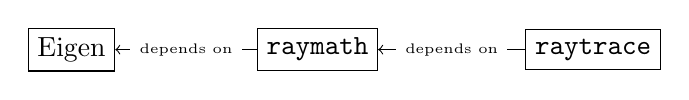
\begin{tikzpicture}
      \node[shape=rectangle,draw=black] (e) at (-3.125,0) {Eigen};
      \node[shape=rectangle,draw=black] (rm) at (0,0) {\texttt{raymath}};
      \node[shape=rectangle,draw=black] (rt) at (3.5,0) {\texttt{raytrace}};

      \path [<-](e) edge node[midway, fill=white] {\tiny depends on} (rm);
      \path [<-](rm) edge node[midway, fill=white] {\tiny depends on} (rt);
  \end{tikzpicture}
  \caption{Component and dependency relationships in \texttt{rayterm-cpu}}
  \label{fig:rayterm-cpu-components}
\end{figure}

Eigen \cite{eigenweb} is a linear algebra for C++ that supports matrix and vector manupulations, various matrix decompositions and geometry features, and has many extensions for numerous other numerical operations.
Eigen is also extremely well-optimized and uses SSE vectorized code, vastly improving performance on supported CPUs.
In \texttt{raymath}, Eigen is used primarily for easy, tested representations and calculations involving vectors; all of the algorithms implemented use equations derived from the ones in Section~\ref{ch:intro:background:raytracing_math}, and so benefit from easy implementation.

The base component in \texttt{rayterm-cpu} -- \texttt{raymath} -- provides support for various geometries and intersection routines. The geometries supported can be seen in Figure~\ref{fig:rayterm-cpu-raymath-geometry}, and use Eigen structures to represent their geometric data.
\texttt{raymath} also handles random number and vector generation, color handling, and intersection representation.
The implementations behind these are covered in Section~\ref{ch:implementation:rayterm-cpu:raymath}.

\begin{figure}[htb]
  \centering
  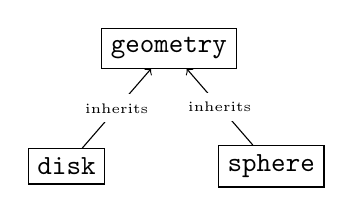
\begin{tikzpicture}
    \node[shape=rectangle,draw=black] (g) at (0,1.5) {\texttt{geometry}};
      \node[shape=rectangle,draw=black] (s) at (1.3,0) {\texttt{sphere}};
      \node[shape=rectangle,draw=black] (d) at (-1.3,0) {\texttt{disk}};

      \path [<-](g) edge node[midway, fill=white] {\tiny inherits} (s);
      \path [<-](g) edge node[midway, fill=white] {\tiny inherits} (d);
  \end{tikzpicture}
  \caption{Geometric structures in \texttt{raymath}}
  \label{fig:rayterm-cpu-raymath-geometry}
\end{figure}

The main component in \texttt{rayterm-cpu} is \texttt{raytrace}; it handles world representation, materials, and raytracing.
\texttt{rayterm-cpu} only renders in \texttt{ppm} mode, since the Tickit interface was only integrated in the \texttt{rayterm-gpu} implementation, since that was the final prototype.
\texttt{raytrace} represents objects with a \texttt{WorldObject} class, a list of which is stored in a \texttt{World}.

Figure~\ref{fig:rayterm-cpu-raytrace-journey-of-a-ray} shows the function call path that is used when rendering a single ray.
The main entry point is \texttt{raytrace\_ppm}, which creates rays with a \texttt{Camera} class instance.
This instance contains specific parameters to control the position and orientation of the virtual camera, and thus controls where the \texttt{ray} originates from. and its direction.
Then, that \texttt{ray} is sent on to the \texttt{World} class, where an \texttt{intersection} is retrieved, and then used to generate a \texttt{color} from the given \texttt{ray}.
This color is then finally returned to \texttt{raytrace\_ppm}, which writes it to a \texttt{ppm} file.
Unmentioned in this diagram are the recursive calls to \texttt{World::trace} from from \texttt{WorldObject::colorize}, which use the transformed ``scatter'' \texttt{ray} from \texttt{Material::scatter}.
The implementation behind all of these structures and functions are covered in Section~\ref{ch:implementation:rayterm-cpu:raytrace}.

\begin{figure}[htb]
  \centering
  \begin{tikzpicture}
    \node[shape=rectangle, draw=black] (a) at (0,0) {Ray collection in \texttt{raytrace\_ppm}};
    \node[shape=rectangle, draw=black, right = 2.5em of a ] (b) {Generation in \texttt{Camera::get\_screen\_ray}};
    \node[shape=rectangle, draw=black, below = 1.75em of a] (c) {World tracing in \texttt{World::trace}};
    \node[shape=rectangle, draw=black, right = 2.5em of c] (e) {Ray coloring in \texttt{WorldObject::colorize}};
    \node[shape=rectangle, draw=black, below = 1.75em of e] (s) {Ray scattering in \texttt{Material::scatter}};
    \node[shape=rectangle, draw=black, below = 1.75em of c] (d) {World intersection in \texttt{World::intersects}};
    \begin{scope}[xshift=1cm]
      \node[shape=rectangle, draw=black] (f) at (2.75, -4.15) {Object intersection in \texttt{WorldObject::intersects}};
      \node[shape=rectangle, draw=black, below = 1.75em of f] (g) {Geometry intersection in \texttt{geometry::intersects}};
      \path [->](d) edge node[midway, fill=white] {\tiny calls} (f);
      \path [->](f) edge node[midway, fill=white] {\tiny calls} (g);
    \end{scope}

      \path [->](a) edge node[midway, fill=white] {\tiny calls} (b);
      \path [->](a) edge node[midway, fill=white] {\tiny calls} (c);
      \path [->](c) edge node[midway, fill=white] {\tiny calls} (d);
      \path [->](c) edge node[midway, fill=white] {\tiny calls} (e);
      \path [->](e) edge node[midway, fill=white] {\tiny calls} (s);
  \end{tikzpicture}
  \caption{The journey of a \texttt{ray} and its \texttt{intersection}}
  \label{fig:rayterm-cpu-raytrace-journey-of-a-ray}
\end{figure}

\littlesection{Algorithms} \label{ch:methods:renderer:sequential:algorithms}

The sequential renderer implements single-branch Monte Carlo ray-tracing, a type of rendering that can produce physically accurate images with little development effort.
The algorithm is largely based on randomness, only modifying the path of a single ray as it bounces around the scene.
When encountering objects, a particular Probability Distribution Function (PDF) is used to calculate where the ray will bounce.
These PDFs vary based on the material, and are hardcoded in the \texttt{Material} implementation.
The result of this algorithm is extremely noisy because of this randomness (see Figure~\ref{fig:rayterm-cpu-ppm-noisy}), so many samples must be taken and then averaged to gain a true value for a single pixel; this simulates the many millions of photons that would have traveled to that pixel in a real camera.
The number of samples per pixel, sometimes termed ``spp,'' is the number of rays generated from a random origin within the pixel.
An example of various spp values is shown in Figure~\ref{fig:rayterm-cpu-ppm-noisy}.

\begin{figure}[htb]
  \centering
  \begin{subfigure}[htb]{0.45\textwidth}
    \includegraphics[width=\textwidth]{impl-images/comparisons/samples_spp_1}
    \caption{1 sample per pixel}
    \label{fig:rayterm-cpu-ppm-noisy-1}
  \end{subfigure}
  \hspace{1em}
  \begin{subfigure}[htb]{0.45\textwidth}
    \includegraphics[width=\textwidth]{impl-images/comparisons/samples_spp_4}
    \caption{4 samples per pixel}
    \label{fig:rayterm-cpu-ppm-noisy-4}
  \end{subfigure}
  \vspace{1em}
  \begin{subfigure}[htb]{0.45\textwidth}
    \includegraphics[width=\textwidth]{impl-images/comparisons/samples_spp_32}
    \caption{32 samples per pixel}
    \label{fig:rayterm-cpu-ppm-noisy-32}
  \end{subfigure}
  \hspace{1em}
  \begin{subfigure}[htb]{0.45\textwidth}
    \includegraphics[width=\textwidth]{impl-images/comparisons/samples_spp_1024}
    \caption{1024 samples per pixel}
    \label{fig:rayterm-cpu-ppm-noisy-1024}
  \end{subfigure}
  \caption{Sample per pixel differentiated output from \texttt{rayterm-cpu}}
  \label{fig:rayterm-cpu-ppm-noisy}
\end{figure}

\littlesection{Prototype} \label{ch:methods:renderer:sequential:prototype}

This section describes the lessons learned from CPU implementation, and how the GPU implementation will differ and improve because of this step.

The final implementation of \texttt{rayterm-cpu} only renders images through a Google Test \cite{googletest} case, which can be run with the \texttt{test.sh} script in the implementation repository \cite{raytermCpuImpl}, or \texttt{gradle test}.
This generates a \texttt{test\_image.ppm} file, examples of which we show from various stages of development in Section~\ref{ch:implementation:rayterm-cpu:raytrace}.
Because of this, \texttt{rayterm-cpu} is very much a proof-of-concept and learning example, rather than a fully-fledged library.

\subsection{Parallel} \label{ch:methods:renderer:parallel}

After the implementation of \texttt{rayterm-cpu}, more performance was needed for the final \name\ implementation.
The solution to this problem was to use a Graphics Processing Unit (GPU) to drastically parallellize the raytracing algorithm.
This improves performance dramatically, because each eye-ray's children (the result of a collision between an object and a ray) are dependant on only their parent eye-ray.
Thus, the computation of a single pixel's color is completely independent of every other pixel.

A short introduction to GPUs may be useful here; they consist primarily of small units of computation circuitry called ``multiprocessors'' which themselves are controllers for several CUDA cores \cite{fermi2009nvidia}, distributing workloads.
These CUDA cores execute individual threads on the GPU, and act somewhat like advanced floating point arithmatic computation units.
A discussion on the specific hardware used for development and testing is available in Section~\ref{ch:intro:background:hardware}.

With 227 commits and over 1.5 thousand lines of code, along with many thousands of additions and deletions, \texttt{rayterm-gpu} has a good start on its life.
There are many, many more improvements possible, however.
We detail some of them in the context of the larger \name\ implementation in Section~\ref{ch:methods:threats}.

\littlesection{Libraries} \label{ch:methods:renderer:parallel:libraries}

This section talks about OptiX and CUDA.

\littlesection{Design} \label{ch:methods:renderer:parallel:design}

This section is about the code structure and organization in the \texttt{rayterm} implementation.

\littlesection{Demonstration} \label{ch:methods:renderer:parallel:demo}

This is a demonstration section on final renderer is capabable of -- this section uses only \texttt{ppm} output.

\section{Interface Implementation} \label{ch:methods:interface}

\subsection{Design} \label{ch:methods:interface:design}
 % Chapter organization is topic-dependent

%ch:implem
%
% $Id: ch04_implementation.tex
%
%   *******************************************************************
%   * SEE THE MAIN FILE "AllegThesis.tex" FOR MORE INFORMATION.       *
%   *******************************************************************
%
\chapter{Implementation}\label{ch:implementation}

\section{\texttt{rayterm-cpu}}\label{ch:implementation:rayterm-cpu}

\subsection{\texttt{raymath}}\label{ch:implementation:rayterm-cpu:raymath}

\subsection{\texttt{raytrace}}\label{ch:implementation:rayterm-cpu:raytrace}


\section{\texttt{rayterm-gpu}}\label{ch:implementation:rayterm-cpu}
% \subsection{}\label{ch:implementation:rayterm-cpu:raytrace}

\section{Challenges}

CPU:
\begin{enumerate}
  \item metal bug
  \item blender comparisons
  \item space differential
  \item coordinate systems
  \item research difficulty (can't read a physics textbook for each material)
\end{enumerate}

GPU:
\begin{enumerate}
  \item Travis testing
  \item library management
  \item gradle integration
  \item [...]
\end{enumerate}
 % Chapter organization is topic-dependent

% YOU MAY HAVE SEVERAL MORE CHAPTERS, DEPENDING ON TOPIC AND ORGANIZATION

%ch:conclusion
%
% $Id: conclusion.tex
%
%   *******************************************************************
%   * SEE THE MAIN FILE "AllegThesis.tex" FOR MORE INFORMATION.       *
%   *******************************************************************
%

\chapter{Discussion and Future Work}\label{ch:conclusion}

\section{Summary of Results}\label{ch:conclusion:summary}

\section{Future Work}\label{ch:conclusion:future}

\begin{enumerate}
  \item more materials / MDL support
  \item scene description language
  \item better rtexplore movement
  \item environment image mapping (missed rays => image lookup)
  \item much more...
\end{enumerate}

\section{Conclusion}\label{ch:conclusion:end}

\name\ is a complex system, the implementation and design of which is an ongoing process.
The system currently supports real-time 3D scene viewing through a terminal emulator.
This is made possible through the OptiX library allowing ray-surface intersection calculations to be done a highly parallelized manner on a GPU.
The Tickit interface and its half-pixel translation algorithm, along with \texttt{libtickit} itself, enable \name\ to treat a terminal as an image canvas.
\name\ is now a fully real-time capable ray-tracing engine, rendering 30 or more Unicode character images per second to a terminal window on a moderately powerful computer.
Since the initial startup development of \name\ is complete, all contributions to \name\ development are now welcome.
In pursuit of maintaining good open-source readability and ease of development, documentation has been and will continue to be a priority throughout the transition process.
We hope that future projects find \name\ inspiring and useful, whether as an engine or as a jumping-off point for real-time ray-tracing and terminal-based games.
 % Conclusion/future work

%   ********************************************************************
%   * IF YOU HAVE ANY APPENDICES (FOR INSTANCE, CODE, DATA, GRAPHS,    *
%   * OR ANYTHING ELSE THAT DOESN'T "FIT" AS REGULAR CHAPTER CONTENT), *
%   * INCLUDE THE FOLLOWING LINE, WHICH INSTRUCTS LATEX TO CHANGE FROM *
%   * NUMBERED "CHAPTER" HEADINGS TO LETTERED "APPENDIX" HEADINGS.     *
%   *                                                                  *
%   * APPENDICES HAVE THE SAME FORMATTING COMMANDS AS CHAPTERS (E.G.,  *
%   * "\chapter{...}", "\section{...}", ETC.)                          *
%   ********************************************************************

\appendix

%
% $Id: appa--code
%
%   *******************************************************************
%   * SEE THE MAIN FILE "AllegThesis.tex" FOR MORE INFORMATION.       *
%   *******************************************************************

\chapter{Code}\label{appendix:code}
This appendix lists some miscellaneous code snippets.
However, the main body of work for \name\ is located in two GitHub repsitories, listed in the bibliography as \cite{raytermCpuImpl} and \cite{raytermGpuImpl}.


\section{Time Multiplication Operations}\label{appendix:timemul}
\lstinputlisting[language=C++]{code/timemul.cpp}

\chapter{Larger Figures}\label{appendix:large_figures}
This appendix shows larger images for some figures.

\vspace{0.3em}
\begin{figure}[htb]
  \centering
  \begin{subfigure}[htb]{\textwidth}
    \includegraphics[width=\textwidth]{impl-images/comparisons/before_smooth_normals}
    \caption{Geometric normals (unsmoothed)}
    \label{fig:rayterm-gpu_unsmoothed_normals_large}
  \end{subfigure}
  \begin{subfigure}[htb]{\textwidth}
    \includegraphics[width=\textwidth]{impl-images/comparisons/after_smooth_normals}
    \caption{Interpolated normals (smoothed)}
    \label{fig:rayterm-gpu_smoothed_normals_large}
  \end{subfigure}
  \caption{Comparison of geometric and interpolated normals}
  \label{fig:rayterm-gpu_smooth_normal_comparison_large}
\end{figure}

%   *******************************************************************
%   * SEE THE MAIN FILE "AllegThesis.tex" FOR THE "\lstset" COMMAND   *
%   * THAT DEFINES HOW PROGRAM LISTINGS WILL LOOK.                    *
%   *******************************************************************
  % Appendices go here

%   ********************************************************************
%   * THE FINAL COMMANDS DEAL WITH BIBLIOGRAPHY/REFERENCES. IF THERE   *
%   * ARE ANY ITEMS IN YOUR BIBTEX FILE THAT YOU DID NOT REFERENCE IN  *
%   * YOUR PAPER, BUT THAT YOU WISH TO INCLUDE IN THE BIBLIOGRAPHY,    *
%   * YOU MAY SPECIFY "\nocite" COMMANDS TO FORCE THEM TO BE INCLUDED. *
%   *                                                                  *
%   * THE COMMAND "\nocite{*}" FORCES EVERY ITEM IN YOUR BIBTEX FILE.  *
%   ********************************************************************

\nocite{*}


\begin{spacing}{1}
\bibliographystyle{plain}
\bibliography{AllegThesis}
\end{spacing}

\typeout{THEPAGE \thepage}

\end{document}
